\chapter{Zero-Knowledge Proofs}
This chapter surveys selective literature about zero-knowledge proofs for practical design applications. The goal is to familiarize the reader with the content classification of zero-knowledge proofs in cryptography and to give an introduction and comparison of the central argument systems widely used today. 

Zero-knowledge proof systems belong to the domain of verifiable computation \citep{Simunic, Ahmad}. Verifiable computation (VC) uses cryptographic protocols and arguments to verify that a computation was performed correctly. The introduction of interactive proof systems (\acrshort{ip}s) by \citet{GoldwasserIPs} and \citet{BabaiIPs} shows that only correct proofs are valid and malicious proving strategies cannot be verified. Traditional proofs are static and are made for easy, step-wise computation verification, whereas \acrshort{ip}s require interaction between the prover and verifier. In computational complexity theory, interactive proof systems are abstract machines exchanging messages between the prover and verifier to convince the verifier that these strings belong to a language \(L\). Here, the formal language \(L\) defines a decision problem, but i.e., a computational problem with binary classification, yes and no. Examples of sets of strings in \(L\) can be that a specific Bitcoin transaction is valid, \(x = 7\) for a given \(f(x)\), or a particular object belonging to a specific Merkle tree. The untrusted prover has unlimited computational power, and the verifier is honest and computationally restricted. 

Advances in computational complexity theory during that time showed that \acrshort{ip}s are more efficient and belong to a broader class than the traditional NP, i.e., problems solvable in deterministic polynomial time by reading proof strings of polynomial length \citep{IOPsdisc}. In 1987, it has been shown that every language belonging to NP has zero-knowledge proof systems \citep{anymental10.1145/28395.28420}. Later, it has been proven that the class of \acrshort{ip}, i.e., problems solvable by interactive proof systems, lies in PSPACE, i.e., problems solvable in polynomial space \citep{Shamir10.1145/146585.146609} and that every language \(L\) in polynomial time has an interactive proof system \citep{Lund10.1145/146585.146605}. The complexity class of \acrshort{ip} describes prover and verifier interaction in a polynomial number of rounds. Other important advances in computational complexity theory are \acrshort{mip}=NEXP \citep{Laszlo} and the \acrshort{pcp} theorem \citep{PCPTheorem}. These works resulted in a set of proof and argument systems that will be introduced in this chapter. \citet{Thaler} gives an exhaustive overview of all systems and in-depth protocol descriptions. 

The following examined proof systems are secure against computationally unrestricted provers: Interactive Proofs (IPs), linear Probabilistically Checkable Proofs (\acrshort{pcp}s), and Interactive Oracle Proofs (\acrshort{iop}s). 

Combining the systems above with cryptographic tools to force specific behavior in the proof generation will create an argument system. Argument systems are considered zero-knowledge if the proof reveals nothing but its validity \citep{GoldwasserIPs}. Adding certain properties, e.g., non-interactivity, succinctness, and knowledge, will design a specific argument of knowledge, e.g., \acrshort{zksnark} (zero-knowledge succinct non-interactive argument of knowledge). Different \acrshort{zksnark}s and notions will be examined in more detail.

The following sub-chapters are structured according to the design-oriented approach described above:
\begin{itemize}
    \item IPs, and \acrshort{iop}s are defined. Through the combination of polynomial commitment schemes or cryptographic tools, argument systems can be designed. Non-interactivity is achieved through the Fiat-Shamir transformation.
    \item Properties and mathematical tools are introduced to describe different arguments of knowledge: \acrshort{zksnark}, \acrshort{fri}-STARK, and bulletproofs. Real-world applications of zero-knowledge proof systems are summarized.
    \item The different proof systems are evaluated according to computational complexity, communication, and security.
\end{itemize}

\section{From Proof Systems towards Argument Systems}

A mathematical proof in the context of computer science and cryptography is any object that convinces a verifier that a statement is correct. Mathematical proofs embody what is defined in the complexity class NP. A proof system is a structured scheme that decides whether a statement is correct or incorrect. Three properties are desirable for proof systems \citep{GoldwasserIPs}, which will be introduced shortly. Throughout this chapter, these properties are revisited more exhaustively.
\begin{itemize}
    \text{\parbox{420pt}{
    \item The procedure to create and verify proofs should be \textbf{efficient and fast}. 
    \item \textbf{Completeness}: True statements should have convincing proof of their validity.
    \item \textbf{Soundness}: If a statement is incorrect, there is no possibility of it having convincing proof.}}
\end{itemize}
Unlike argument systems, proof systems do not limit the malicious prover in its computational power (statistical soundness). Using cryptographic primitives and restricting the prover, e.g., probabilistic polynomial time proof, so that it cannot break the primitives, describes the design towards argument systems, which are computationally sound \citep{ArgSystems, MicaliArgSys}. Each proof system presented makes assumptions about the prover. However, only with cryptographic tools and zero knowledge can these proof systems be extended with additional properties to yield zero-knowledge argument systems of various kinds.

\subsection{Interactive Proofs}
In interactive proof systems, the prover with unlimited computational resources interacts with a computationally bound verifier to convince the verifier of the correctness of a statement. The verifier randomly challenges the prover, which is called coin tosses \citep{GoldwasserCoinTosses}. These challenges happen in rounds until sufficient tests are run, and the verifier is convinced. \citet{GoldwasserIPs} defined an interactive proof system that is private, i.e., that the verifier's challenges are not publicly accessible, whereas the interactive proof system of \citet{BabaiIPs} allows the coin tosses to be publicly accessible by the prover.
\begin{align*}
    \text{\parbox{450pt}{\textbf{Interactive Proof System.} \textit{\(L\) is a language over \(\{0,1\}^n\), with n representing the input size domain of n-bit strings. An interactive protocol is an interactive proof system if, after \(k\) rounds, the probabilistic verifier in polynomial time exchanged \(k\) messages with the computationally unrestricted prover and has to either accept or decline the correctness of the prover's proposition. IP is the complexity class of problems solvable by a k-round interactive proof system.}}}
\end{align*}
The transcript is the order in which messages are exchanged. The prover and verifier are functions \(P(x), V(x)\) with common input \(x\). The overall distribution of all transcriptions between the prover and verifier is called \(View_V(P(x), V(x))\), which is bound by the number of rounds between \(P\) and \(V\). \(P\) provides a result that satisfies the proposition, e.g., \(y\) to a function \(f(x) = y\). \(P\) and \(V\) exchange a transcript of messages \((m_1, m_2, m_3, ..., m_k)\), whereby both parties take turns, and the prover sends the last message. Note that \(V\) is probabilistic with internal randomness \(r\). Hence, the output depends on \((V, x, r, P)\) and is \(\{0,1\}\), i.e., \(1\) if the statement is correct, and \(0\) if it is incorrect \citep{GoldwasserIPs, BabaiIPs}. Interactive proof systems have completeness error \(\delta_c\) and soundness error \(\delta_s\) . For any input \(x\), there must be a convincing proof that \(f(x)\) is correct. Incorrect statements for \(y \neq f(x)\) cannot result in a convincing proof, i.e., a malicious prover does not exist. \acrshort{ip} systems are valid if \(\delta_c, \delta_s \leq 1/3\) \citep{Thaler}. \acrshort{ip}s with \(k\) provers are multi-prover interactive proofs (\acrshort{mip}s), introduced by \citet{MIPsBen} and extended by \citet{MIPsSetty} to allow for the design of succinct arguments. \acrshort{mip}s are characterized by no information sharing and non-adaptivity of provers. The probabilistic polynomial time verifier acts similarly as in \acrshort{ip}s, but the challenges sent are not shared among the different provers. The prover's response \(i\) does not depend on the \(i-1\) interactions in the transcript, i.e., the prover cannot react based on the previous messages, because there is at least another prover \(p_j\) whose messages are not known to \(p_i\) for \(i\neq j\).

\begin{comment}
Some definitions are still missing:
randomness
completeness
soundness
statistical soundness
computational soundness
\end{comment}

\subsubsection{Non-interactive, Publicly Verifiable Arguments}
The Fiat-Shamir transformation transforms any interactive proof system based on public coin tosses into a non-interactive, publicly verifiable system. This transformation can be described effectively with the use of an ideal cryptographic assumption, the random oracle model (\acrshort{rom}). 
\subsubsection{Random Oracle Model}
The\acrshort{rom}methodology was introduced in cryptographic theory to satisfy the goal of designing secure cryptographic protocols. First, an ideal system is designed to give all parties access to an oracle, i.e., a random public function. Once the security of the protocol is proven, the random oracle function is replaced by a cryptographic hashing function to implement the system in practice \citep{ROMBellare}. In \acrshort{ip}s, the random oracle function is part of the view, i.e., random choices of challenges simulator output. It is assumed that the prover and verifier can query the random oracle function \(f_R\) by sending an input \(x\) so that the random oracle returns \(f_R(x)\). In \acrshort{rom}, the efficiency is dependent on x, i.e., for every input in the problem size domain \(D\), \(f_R(x)\) is captured. Since it is only practical in theory, because \(|D|\) is large to ensure security, e.g., \(2^{256}\), hash functions are used in practice \citep{ROMBellare, Thaler}, e.g., POSEIDON or SHA-3. The \acrshort{rom} is controversially discussed in retrospect: On the one hand, it is argued that there exist protocols that are only secure in the \acrshort{rom}, and all implementation efforts in practice have led to insecure protocols, whereby the security of the ideal scheme is not maintained. The area of work at focus is digital signatures and public-key encryption, showing that the \acrshort{rom} is not sound \citep{ROMCanetti}. On the other hand, this conclusion is discussed to indicate there is no evidence of practical security weaknesses if there is a need for random oracle systems in a protocol. Protocol design examples support this statement, e.g., Elliptic Curve Digital Signature Algorithm (ECDSA), leading to cryptographic insecurity if not using a random oracle \citep{ROMretroKoblitz}. 
\subsubsection{Fiat-Shamir Transformation}
The Fiat-Shamir transformation (\acrshort{fst}) \citep{ROMFiat1986HowTP} removes the need for prover-verifier interaction in a public coin interactive proof system with the help of the random oracle function. The result is a non-interactive, publicly verifiable system. \acrshort{ip}s send messages between the prover and verifier, whereby the verifier challenges the prover randomly. Every message the verifier sends in the \acrshort{ip} is replaced by values obtained by querying the random oracle. The query always depends on the previous message sent by the prover to prevent soundness attacks.

In summary, the prover only sends one message containing the transcript, i.e., the list of all messages sent by the prover and the query results of the random oracle. The input x has to be appended to the list every round. The verifier's coin tosses are no longer needed, and the verifier does not need to send messages to the prover (Figure \ref{fig:FST}).
\begin{figure}[hbt]
	\centering
		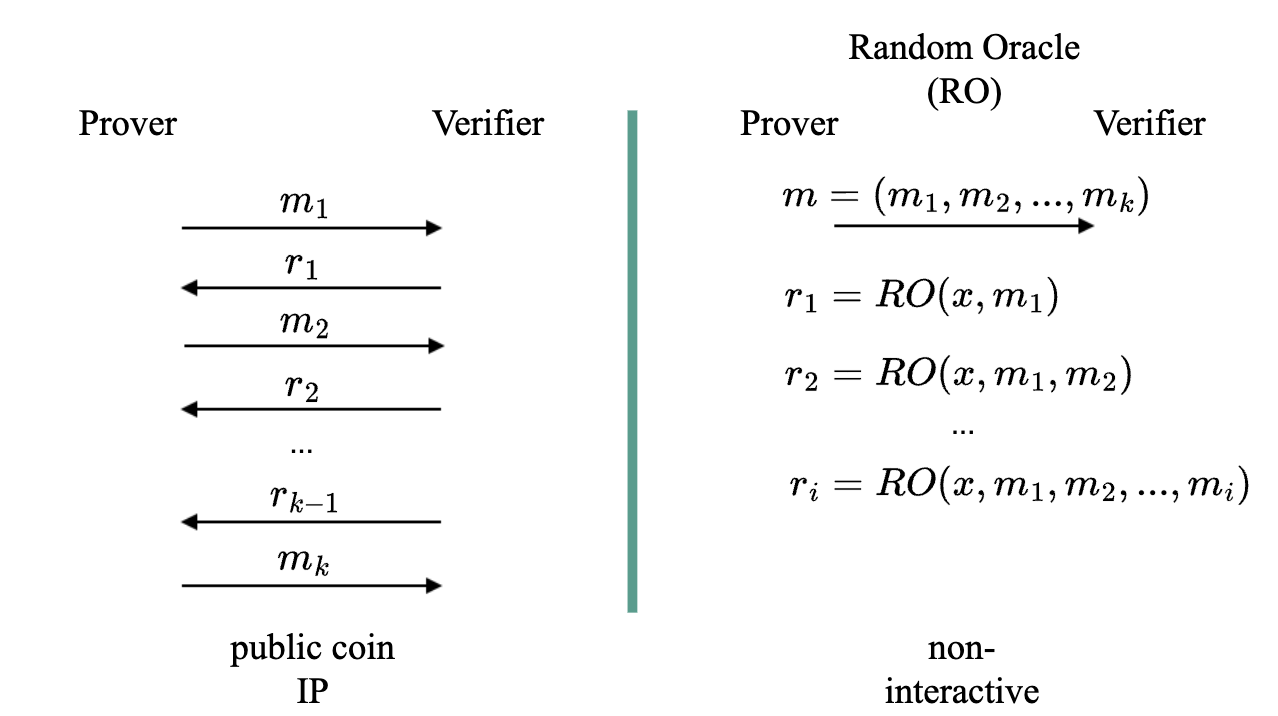
\includegraphics[width=0.7\textwidth]{Pictures/FST.png}
	\caption{Illustration of Generic Fiat Shamir Transformation (based on \citet{Thaler})}
	\label{fig:FST}
\end{figure}
Argument systems are obtained by applying polynomial commitment schemes to proof systems, while the prover commits to a low-degree polynomial. It allows for polynomial evaluation verification without possessing all the information of this polynomial. Polynomial commitment schemes are used to prove that a polynomial, evaluated at a specific input, results in a specific output. The prover commits to the polynomial, acting as some object hiding the polynomial, e.g., similar to a hash. The verifier challenges the commitment with a random value. The committer then creates a proof that the polynomial evaluates at that random value at a specific point. The polynomial itself is not revealed. In interactive proof systems with an honest prover running in polynomial time, any arithmetic circuit can be evaluated \citep{GKR10.1145/1374376.1374396}. Arithmetic circuits have gates that operate on two types, i.e., addition and multiplication. Besides gates, some wires carry integer variables. Retrospectively, it is a significant achievement since arbitrary computer programs can be expressed via arithmetic circuits, the base layer of many zero-knowledge protocols today. More mathematical tools for understanding the functionality of argument systems are covered in Chapter 4.2.
\subsubsection{Zero-Knowledge}
If the verifier knows nothing about the statement and the witness but its validity, the algorithm will run with zero knowledge. This property can be described by using a simulator notion \citep{Thaler}: A prover and probabilistic polynomial time verifier strategy exists under the honest verifier assumption. For any probabilistic polynomial time verifier strategy, there is a probabilistic polynomial time algorithm (simulator) that can depend on the verifier strategy, which produces outputs that are indistinguishable from the distribution of transcripts generated through the prover and verifier strategy interactions. The simulator ensures that the verifier only learns that \(x \in L\). Under the honest verifier assumption, there are at least six types of zero-knowledge protocols, whereby the notion of simulator output and transcript distribution being indistinguishable is at focus \citep{zktypes}:
\begin{itemize}
    \item \textbf{Perfect Zero-Knowledge}: The output of the simulator \(S(x)\) and the distribution of the transcript created through prover and verifier strategy interaction \(View_V(P(x), V(x))\) within the protocol is identical. 
    \item \textbf{Statistical Zero-Knowledge}: \(S(x) \text{ and } View_V(P(x), V(x))\) have a negligible statistical distance, given a polynomial number of samples from the distributions.
    \item \textbf{Computational Zero-Knowledge}: \(S(x) \text{ and } View_V(P(x), V(x))\) can be distinguished with negligible probability only if a polynomial number of samples is given.
\end{itemize}
Soundness is divided into statistical (for proof systems) and computational (for argument systems) soundness. Argument systems are computationally sound, i.e., allow for applying cryptographic primitives. The computationally bound prover cannot break these primitives, unlike the unbound prover in proof systems, which are statistically sound \citep{Thaler}. The verifier learns that a statement is true and has to be convinced that the prover knows a correct witness. The simulator is able to extract that witness information through interaction with the algorithm (knowledge soundness) \citep{NitulescuGentleIntroSNARKs}.

\subsection{Linear Probabilistically Checkable Proofs}
Probabilistically checkable proofs (\acrshort{pcp}s) differ from previously introduced proofs because the prover does not need to answer queries based on the current or previous query content posted by the verifier. The polynomial time verifier is provided with oracle access to a static proof string \begin{math} \pi \end{math}, whereby the proof is queried, and the result of it only depends on the currently processed query \citep{PCP}. The breakthrough of robust, pairing-based schemes is attributable to \citet{GennaroLinPCP}, who introduced Quadratic Arithmetic Programs (\acrshort{qap}s) as a variant of quadratic span programs. Quadratic span programs are efficient because they only satisfy boolean circuits. Therefore, introducing \acrshort{qap}s is essential to represent more practical computations, e.g., multiplication gates, whereby the efficiency lies in the usability for effectively solving more natural problems. Any arithmetic circuit instance can be transformed into instances of a rank-1 constraint system (\acrshort{r1cs}).
\begin{align*}
    \text{\parbox{450pt}{\textbf{\acrshort{r1cs}.} \textit{A \acrshort{r1cs} is an intermediate representation of the computational problem, which is used to perform the application of argument systems. Given a set of \(n \times m \text{ matrices} \ A, B, C\), with values derived from a finite field \begin{math} \mathbb{F} \end{math}. An \acrshort{r1cs} instance is called satisfiable if there exists a solution vector \(z \in\) \begin{math} \mathbb{F}^n \end{math} with \(z_1 = 1\), so that}}}
\end{align*}
\begin{align*}
    (A \cdot z) \circ (B \cdot z) = C \cdot z.
\end{align*}
For every \(i\)th row of each of the three matrices belonging to the finite field circuit size, the following equation must hold:
\begin{align}
    \langle a_i, z \rangle \cdot \langle b_i, z \rangle - \langle c_i, z\rangle = 0 
\end{align}

In practice, \(z\) is known by the prover. The solution vector also has a public input, namely the computation result (refer to Chapter 5.2 for an example calculations). The goal is to arrive at a univariate polynomial \(t(x)\) when divided by the minimal polynomial, represents a secret polynomial \(h(x)\) without remainder. The minimal polynomial is always known if the number of constraints is known and is a multiple of \(t(x)\). The linear \acrshort{pcp} is evaluated in linear, constant time. The \acrshort{qap} is obtained by taking each value of each row of the \acrshort{r1cs} matrices as an output of a polynomial, which is to be calculated. The polynomial results to that specific value in the \acrshort{r1cs}, when evaluated at \(X = \{1, 2, ..., \text{number of constraints}\}\). Given these constraints, the three sets of polynomials are calculated via the sum of Lagrange Interpolation.
\begin{align*}
    \text{\parbox{450pt}{\textbf{Lagrange Interpolation.} \textit{The polynomial obtained through Lagrange Interpolation is the polynomial \(P(x)\) of degree at most \(\leq (n-1)\) and passes through the n points \((x_1, y_1 = f(x_1)), (x_2, y_2 = f(x_2), ..., (x_n, y_n = f(x_n))\), that are given. It is denoted by}}}
\end{align*}
\begin{align}
        P(x) = \sum_{j=1}^{n} P_j(x)
\end{align}
\begin{align*}
        P_j(x) = y_j * \prod_{\substack{k = 1 \\ k \neq j}}^{n}\frac{x-x_k}{x_j-x_k}
\end{align*}
\begin{align*}
    \text{\parbox{450pt}{\textbf{Example.} \textit{Let \(n = 2\) with the three given points \([1,0], [2,1], [3,0]\). The polynomial obtained through Lagrange Interpolation is: 
    }}}
\end{align*}
\begin{align*}
    P(x) = \sum_{j=1}^{2}\left(y_j*\prod_{\substack{k = 1 \\ k \neq j}}^{n}\frac{x-x_k}{x_j-x_k}\right)
    &= 0 * \frac{(x-2)(x-3)}{(1-2)(1-3)}+1*\frac{(x-1)(x-3)}{(2-1)(2-3)}\\
    &= 0 * \frac{(x-1)(x-2)}{(3-1)(3-2)} = \frac{x^2-4x+3}{-1}\\
    &= -x^2+4x-3
\end{align*}
Each gate is the \(x\) value, and the values of the \acrshort{r1cs} matrix column are the corresponding \(y\) values for the computation to obtain the \acrshort{qap}. It consists of three sets of polynomials (Chapter 5.2). Each interpolation calculation receives \(n\) points (number of constraints), and the result is a polynomial of degree \(n-1\). Multiplying each polynomial in the matrices with the solution vector yields the final polynomials \(A(x), B(x), C(x)\) and
\begin{align}
    \frac{A(x) * B(x) - C_(x)}{Z(x)} = H(x).
\end{align}
In a linear \acrshort{pcp}, the proof consists of evaluations of linear functions created by the prover. Soundness is guaranteed against a dishonest prover by ensuring the proofs rely on a specific structure. The verifier is querying the proof by transforming linear \acrshort{pcp}s into non-interactive argument systems. The trusted set-up issues proving and verifying keys, which are used to perform checks using pairing-based cryptography. Many systems rely on this feature, e.g., Groth16, whose mathematical tools and general protocol procedures are presented in Chapter 4.2.1.

\subsection{Interactive Oracle Proofs}
Interactive oracle proofs (\acrshort{iop}s) can generalize \acrshort{pcp}s and \acrshort{ip}s, which decreases the large proof size, e.g., resulting from \acrshort{pcp}s. Introduced by \citet{IOPsdisc}, \acrshort{iop}s are interactive proofs with a verifier receiving query access to the proof in every round instead of the full proof size. The verifier chooses the element of the message in every round and only pays the cost of the query, which results in a verifier time that is sub-linear to the total proof length. \acrshort{iop}s were made non-interactive by introducing Merkle hashing and the \acrshort{fst} in the random oracle model \citep{IOPsdisc}. The prover message is not sent in every round. Instead, the Merkle commitment of the prover's message is sent. The verifier determines which element of the message will be queried through simulation. The prover reveals the relevant element by provisioning the verifier with authentication paths in the Merkle tree. The interactive argument is then transformed into a non-interactive argument via \acrshort{fst}, while soundness is preserved \citep{Thaler}.

SNARKs from constant-round \acrshort{iop}s are slower than \acrshort{ip} or \acrshort{mip}-based \acrshort{iop}s because constant-round \acrshort{iop}s require provers to commit to many polynomials, while in \acrshort{ip} and \acrshort{mip}-based argument systems, provers commit only to a single polynomial. Also, the single polynomial is not larger than any of the many polynomials in constant-round \acrshort{iop}s \citep{IOPconst}. \acrshort{iop}s derived from \acrshort{ip}s and \acrshort{mip}s need recasting to effectively compare the different \acrshort{iop}s because classic \acrshort{ip}s and \acrshort{mip}s use multivariate polynomials. In standard \acrshort{iop}s, each message is sent as a string, and the verifier has to query each string for a specific element. In polynomial \acrshort{iop}s, each message is a polynomial over a finite field \begin{math}\mathbb{F}\end{math} with a degree at most some upper bound specified. Polynomial \acrshort{iop}s for \acrshort{r1cs}-satisfiability use univariate polynomials. These polynomials can have many coefficients, sometimes the size of the \acrshort{r1cs}. If the verifier had read access to the full polynomial description, verifier time would explode to check the proofs \citep{IOPbuenz}. The verifier chooses any input for query access to its evaluation in the specified polynomial. Polynomial commitment schemes are used to obtain succinct arguments so the verifier can confirm that the specified input evaluates to the output received, i.e., that a specific polynomial with a certain degree is correctly specified. Replacing each message and associated evaluation queries with polynomial commitment schemes will make the protocol standard \acrshort{iop}. The transformation steps in \citet{IOPsdisc} will yield succinct arguments for further \acrshort{zkp} design. All SNARKs, except for linear-\acrshort{pcp}-based, are designed according to this approach, e.g., the Fast Reed-Solomon Interactive Oracle Proofs of Proximity (\acrshort{fri}) \acrshort{iop}, an \acrshort{iop}-based polynomial commitment scheme with polylogarithmic proof length (Chapter 4.2.3).

The proof systems introduced in this chapter form the base layer of zero-knowledge succinct, non-interactive arguments of knowledge. The proof is convincing, and the witness is valid. At the same time, the verifier learns nothing about it except its validity; hence cannot be convinced by an invalid witness (completeness, soundness, and zero knowledge).

\section{Zero-Knowledge Succinct, Non-interactive Arguments of Knowledge}
Following the first zero-knowledge \acrshort{ip}s \citep{GoldwasserIPs}, \citet{Blum1991} introduce the common reference string (\acrshort{crs}) and create non-interactive zero-knowledge proofs with only one message to be shared, i.e., the proof. Subsequently, research on reducing the proof size increased, \citet{MicaliArgSys} introduces the first non-interactive zero-knowledge proof with sublinear proof size. Building on these findings, the first \acrshort{zksnark}s for circuit satisfiability uses proofs that are constant-size and uses pairings to efficiently check the polynomial equations without revealing any information, e.g., coefficients \citep{Groth2010ShortPN}. \citet{GennaroLinPCP} continue increasing the efficiency of polynomial equation verification and introducing \acrshort{qap}s. \citet{Pinocchio} makes use of it and develops the Pinocchio protocol, which utilizes \acrshort{qap}s and the knowledge of coefficients to efficiently verify polynomial equations through eight pairing checks without revealing any decodings. This protocol is enhanced by \citet{Groth2016OnTS}, reducing the proof size again and decreasing the number of pairing checks to three. It is widely used today, and the characteristics of succinctness and non-interactivity make it particularly useful in blockchain, e.g., in Zcash and circom \citep{chen2022review}. In the following, different \acrshort{zksnark} designs will be defined. Current research focuses on quantum-resistant systems \citep{chen2022review}.

\subsection{Circuit-specific \acrshort{zksnark} from QAP}
With the introduction of \acrshort{qap} by \citet{GennaroLinPCP} as starting point, \citet{Groth2016OnTS} introduced essential and performative \acrshort{zksnark}s for circuit satisfiability. The linear interactive proof (LIP) provided reduces the number of verifier queries to 3 and the number of group elements from 10 to 6. Previous security relied on the knowledge of exponent assumption, which was enhanced by establishing security in the generic group model. Practically, the Fast Fourier Transform (\acrshort{fft}) is utilized. Changing the circuit to a small degree still requires a complete restart of the trusted set-up \citep{Thaler}. The following introduces preliminary assumptions and definitions for designing circuit-specific \acrshort{zksnark}s from \acrshort{qap}, providing a starting point for the functionalities in the Groth16 protocol applied in Chapter 5.2.
\begin{align*}
    \text{\parbox{450pt}{\textbf{Linear Interactive Proof (LIP).} \textit{While linear \acrshort{pcp}s ensure that the prover answers any verifier query through a linear function, LIPs ensure soundness against provers that do not use the same linear function to answer queries. Any linear \acrshort{pcp} can be transformed to LIP \citep{bitansky}. The Knowledge of Exponent Assumption (\acrshort{kea}) guarantees, under the hard discrete logarithm problem, that the prover is knowledgeable about these linear functions, i.e., can prove that the same coefficients are used for all polynomials resulting from the \acrshort{qap}.}}}
\end{align*}
SNARKs from \acrshort{qap} consist of a generation algorithm, prover, and verifier \citep{Groth2016OnTS, Guo, Benamara}, introduced informally.
The generation algorithm executes the trusted set-up by taking a random security parameter and the arithmetic circuit as input. The \acrshort{qap} is generated over a finite field, which forms the basis for the trusted set-up run. With secret states and parameters not to be known by anyone and deleted after (toxic waste), the \acrshort{crs} is created as an output of the generation algorithm (for detailed structure, see 6.2). The prover algorithm uses the \acrshort{crs} and public statements to compute a witness so that the target polynomial, i.e., the result of encoded computation from \acrshort{qap}, and the minimal polynomial vanish on some quotient polynomial. After it has been ensured, the proof is generated. The proof consists of elements from the encoded computation generated by two group elements. The verifier algorithm uses the proof and performs pairing checks to output either a true or false. In Groth16, the pairing checks are minimal, and the parameters and generated values are mainly taken from the proving and verification keys (Chapter 5.2). Perfect completeness is achieved if the prover knows a true statement because an honest verifier will be convinced \citep{Guo}. Zero-knowledge is achieved by randomizing the polynomials and uniformly distributing the proof terms \citep{Groth2016OnTS, Groth2010ShortPN}.

The combination of linear interactive proofs with pairing-based cryptography is beneficial due to the functionality of bilinear maps (Chapter 5.2). Through the use of bilinear maps, one homomorphic multiplication operation can be executed:
\begin{align*}
    \text{\parbox{450pt}{\textbf{Bilinear Maps and Multiplicative Homomorphism.} \textit{Given the commitments \(a_1, a_2, a_3\) and the values \(b_1, b_2, b_3\) in the commitments, and the bilinearity of the following map \begin{math}
        e: \mathbb{G} \times \mathbb{G} \to \mathbb{G}_t
    \end{math}, \(e(g^{b_1}, g^{b_2}) = e(g^{b_3}, g)\), if and only if \(b_3 = b_1 * b_2\).}}}
\end{align*}
In practice, \begin{math} \mathbb{G} \end{math} is an elliptic curve group defined over a prime finite field \begin{math} \mathbb{F}_p \end{math}, and \begin{math} \mathbb{G}_t \end{math} is a subgroup of the extension field of \begin{math} \mathbb{F}_p \end{math}, namely \begin{math} \mathbb{F}_{p^k} \end{math}. \(k\) is a positive integer and defines the embedding degree of the elliptic curve group, and must be low to apply pairings efficiently. If \(k\) is too large, the mapped elements to \begin{math} \mathbb{G}_t \end{math} will be more expensive to operate on \citep{Thaler}.
\begin{align*}
    \text{\parbox{450pt}{\textbf{Decisional Diffie-Helman Assumption (DDH).} \textit{Given a cyclic group \begin{math}\mathbb{G}\end{math} with generator \(g\) and \(g^a, g^b\) for \(a, b\), chosen uniformly and independently from \begin{math}\mathbb{G}\end{math}, \(g^{ab}\) is computationally indistinguishable from a random group element of the cyclic group.}}}
\end{align*}
Instead of \acrshort{kea}, the \acrshort{fft} can more efficiently compute the Decisional Diffie-Helman problem in \(O(nlogn)\). It is achieved by making use of the roots of unity. The element \(w\) is a root of unity in finite field \begin{math} \mathbb{F}\end{math}, whereby \(w^n = 1\) with \(n\) being the \(n^{th}\) primitive root of unity for all positive integers s smaller than \(n\), \(w^s \neq 1 \). Instead of evaluating a polynomial at \(n\) point pairs \(\{(x_0,y_0), (x_1,y_1), ..., (x_{n-1}, y_{n-1})\}\), the values \(1, w, w^2, ..., w^{n-1}\) are used, halving the values to \(\frac{n}{2}\) \citep{Groth2016OnTS}.

\subsection{Permutation Argument \acrshort{zksnark}}
Permutations over Lagrange-bases for oecumenical non-interactive arguments of knowledge (\acrshort{plonk}) is a \acrshort{zksnark} with a universal trusted set-up, which produces a structured reference string (SRS). The SRS is of size \(d\), used for circuits of up to \(\leq d\) gates. This universal SNARK has fully succinct verification and low prover run time \citep{PLONKcryptoeprint:2019/953}, compared to its predecessor Sonic \citep{SONIC10.1145/3319535.3339817}, which was the first universal and fully succinct SNARK. \acrshort{plonk} is based on constant round polynomial \acrshort{iop} and uses the polynomial commitment scheme based on \citet{Kate2010ConstantSizeCT}. It is presented as a non-interactive protocol obtained through Fiat-Shamir transformation \citep{PLONKcryptoeprint:2019/953}. The trusted set-up is universal and updatable: it can be used for the entire scheme and does not have to be produced for every problem (circuit), e.g., in Groth16. Also, the Kate commitment scheme can be replaced by any other polynomial commitment scheme, e.g., \acrshort{fri} (Chapter 4.2.3). 
Kate commitments use the elliptic curve generated points published in the public key after trusted set-up, similar to Groth16 (Chapter 5.1), to commit to a polynomial of degree \(d\). The first \(d+1\) points are used to evaluate the polynomial at the respective coefficient. The underlying assumptions can be attributed to the Schwartz-Zippel lemma.
\begin{align*}
    \text{\parbox{450pt}{\textbf{Schwartz-Zippel Lemma.} \textit{Let \(f(x)\) be a non-zero polynomial with degree \(d\) over \begin{math}\mathbb{F}^n\end{math}, then, for a randomly chosen \(r\), the probability of \(f(r) = 0\) is at most \(\frac{d}{n}\).}}}
\end{align*}
The Schwartz-Zippel lemma proves that the polynomial evaluates to 0 at any point with high probability if it evaluates to 0 at a given random \(r\). If two polynomials evaluate equally at \(r\), they are equal at every point with high probability. In a polynomial commitment scheme, this suggestion is beneficial. The prover evaluates the polynomial at the random \(r\) chosen by the verifier and sends it along with a proof. If the proof is valid, the verifier concludes that the result of the prover is also valid \citep{Kate2010ConstantSizeCT}.

The computation is first converted into an arithmetic circuit. Then, the arithmetic circuit is used to obtain a constraint system similar to the \acrshort{r1cs} from the previous chapter. Both have only one multiplication allowed per gate. However, if it is not a constant, \acrshort{plonk} only allows for one addition per gate. This constraint system also comes with copy constraints, transforming the system into polynomials. The verification uses a polynomial commitment scheme (Figure \ref{fig:plonk}).

\begin{figure}[hbt]
	\centering
		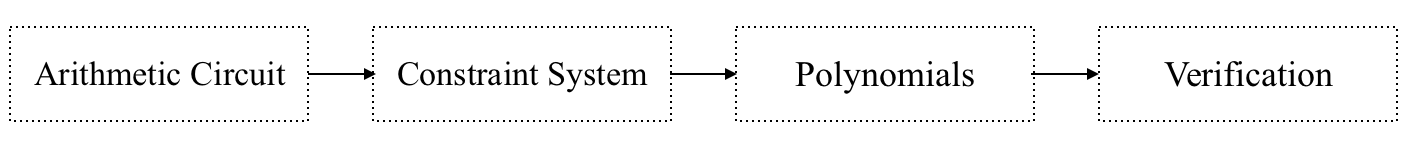
\includegraphics[width=0.8\textwidth]{Pictures/plonk_process.png}
	\caption{\acrshort{plonk} steps (simplified)}
	\label{fig:plonk}
\end{figure}

Like circuit-specific \acrshort{zksnark}s, e.g., Groth16, the computation must be flattened for the protocol to process it. The problem is represented in an arithmetic circuit consisting of gates that can represent an addition or a multiplication. Then, the arithmetic circuit is transformed into a constraint system representing the circuit's wires. In analogy to circuit-specific \acrshort{zksnark}s, the constraint system depends on the number of gates (Chapter 5.2). In \acrshort{plonk}, the constraint system is normalized into a specific form, which will be presented shortly, and is referred to as part of the public input in \citet{PLONKcryptoeprint:2019/953}. 
It is distinguished between constraints per gate and across gates within arithmetic circuits. The formalization system of gate constraints is the following:

\begin{align}
    Q_{L}a + Q_{R}b + Q_{O}c + Q_{M}ab + Q_C = 0
\end{align}

\(L, R, O\) represent the left, right, and output gate wires. \(M, C\) stand for multiplication and constant. This standardized form allows the representation of addition and multiplication. Setting \(Q_{M}ab = 0, \ Q_C=0, \ Q_{O}c = -1 \) and the rest to 1 will represent \(a + b - c = 0\). Setting \(Q_{L}a =1,\ Q_{L}b =1,\ Q_{O}c = -1\) and the rest to 0 will represent multiplication. Each gate is represented in the form presented in 5.1. Similar to the \acrshort{r1cs} previously described, \(Q_{L}a, Q_{L}b, Q_{O}c, Q_{M}ab, Q_C\) can be expressed as vectors that hold the circuit structure. Again, in analogy with the \acrshort{r1cs}, \(a, b, c\) can also be expressed as vectors, which are the witness assignments. In correlation to Chapter 4.2.1 on circuit-specific \acrshort{zksnark}s, these witness assignments might be private and only known to the prover.
In this constraint system, there are vectors \(Q_{L}, Q_{O}, Q_{M}, Q_C, a, b, c\). Using the indices of these vectors as x, they can be transformed into polynomials of evaluation format. For example, let us define one of the vectors in a circuit with 4 gates to illustrate the procedure. 

\begin{align}
    Q_L = (1,0,1,0) \text{ converts into the set of points } {(0,1), (1,0), (2,1), (3,0)}.
\end{align}

The set of points matches a degree 3 polynomial, which can be shown in a coordinate system (Figure \ref{fig:examplepoly}). Through Lagrange Interpolation, the concrete polynomial in coefficient form can be calculated. 
\begin{figure}[hbt]
	\centering
	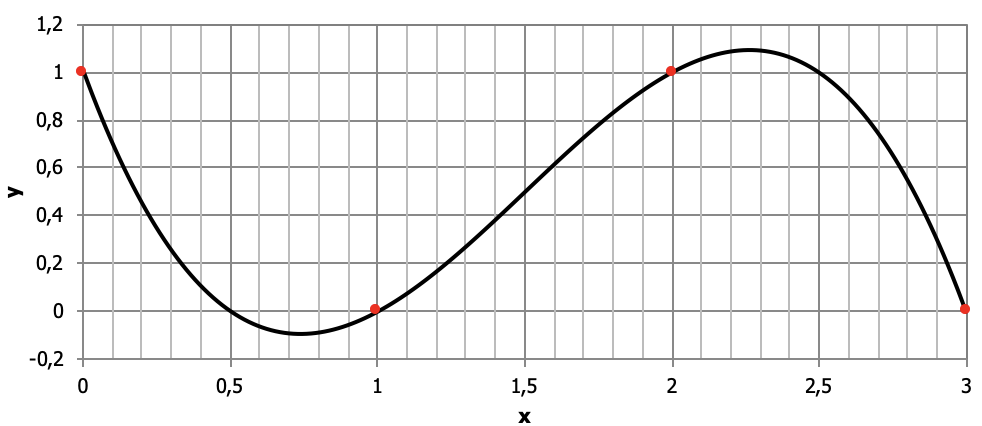
\includegraphics[width=0.6\textwidth]{Pictures/example_polynomial.png}
	\caption{Example polynomial \(Q_{L}(x)\) evaluated at the points in (4.5). Lagrange Interpolation yields coefficient form \(Q_{L}(x) = - 0.6667x^3 + 3x^2 - 3.3333x + 1\)}
	\label{fig:examplepoly}
\end{figure}

This procedure is applied to all Q-vectors and the vectors \(a,\ b,\) and \(c\) to transform them from constants into polynomials. The corresponding function obtained is
\begin{align}
    f(x) = Q_{L}(x)a(x) + Q_{R}(x)b(x) + Q_{O}(x)c(x) + Q_{M}(x)a(x)b(x) + Q_{C}(x) = 0\\
    f(x) = Z(x)H(x)
\end{align}

Now, as much information as possible can be compressed into a single source, i.e., a polynomial. 

Besides the constraints as per gate, some constraints hold across gates, e.g., the output of a gate can be equal to the input on another gate. It is necessary to represent them, too, in order to translate the whole problem into the scheme. These copy constraints can lie within one vector, e.g., if \(b0 = b2\), or between multiple vectors, e.g., \(c0 = a3 = b1\). In the first case, the indices of the vectors are exchanged to create a permutation function \(\sigma(i)\). In the second case, the vectors are combined into one long vector before obtaining the permutation function. Once all copy constraints are generated as lists of permuted indices, they are transformed into polynomials of the permuted gate indices. The resulting polynomials are
\begin{align}
    \sigma_{a}(x), \sigma_{b}(x), \sigma_{c}(x)
\end{align}

A proof is generated by using these permutations and computing the values of all the gates to create the polynomials of \(a(x), b(x), c(x)\). Now, an accumulator \(p(x)\) will be designed in order to represent all coordinates in the set of points between the vectors \(a, b, c\). It proves the copy constraints as follows.
\begin{align}
    p(x+1) = p(x) * (v_1 + X(x) + v_2 * Y(X))
\end{align}
\(v_1, v_2\) are random values and \(X, Y\) are polynomials per vector representing the x and y coordinates. For every copy constraint, e.g., \(a1=a3\) or \(b4=c1\), there will be a \(X(x)\) representing the x coordinates \(a,b, c\). \(X'(x)\) will be a polynomial representing the indices flips in the copy constraint. Every vector will be represented in \(p_{a}(n), p_{b}(n), p_{c}(n)\) and \(p'_{a}(n), p'_{b}(n), p'_{c}(n)\). Instead of checking each copy constraint within the same vector individually, the following multiplication check is also performed to check copy constraints across vectors at the same time:
\begin{align}
    p_{a}(n) * p_{b}(n) * p_{c}(n) = p'_{a}(n) * p'_{b}(n) * p'_{c}(n)
\end{align}
In practice, the permutation accumulators are not expressed in dependency of vector size \(n\) but through high-order roots of unity, whereby the field elements satisfy \(\omega^n = 1\). Also, all values are expressed as elements within a finite field of prime order \(p\), similar to the circuit-specific \acrshort{zksnark}s. The X coordinates are not expressed as indices dependent on vector size \(n\) but with \(omega\) and some random element \(g\) in the field.
\subsubsection{Summary}
After transforming all the constraints intro sets of polynomials, the following checks need to be performed to verify the proofs \citep{PLONKcryptoeprint:2019/953, buterinplonk, chen2022review}. These checks can be verified through the polynomial commitment scheme based on \citep{Kate2010ConstantSizeCT}. Elliptic curve points are generated randomly, similar to circuit-based \acrshort{zksnark}s, and used to evaluate the polynomials. Elliptic curve pairings allow checking whether the equations hold without revealing any generated points or polynomials. 
The equation in (4.3) is the main equation of the circuit that needs to be checked. Then, six permutation accumulator functions exist for the witness assignment vectors and their copy constraints. The equation check in (4.4) results in six rounds:
\begin{align}
    P_{a}(\omega x) - P_{a}(x)(v_1 + x + v_2a(x)) = Z(x)H_{1}(x) \\
    P_{a'}(\omega x) - P_{a'}(x)(v_1 + \sigma_{a}(x) + v_2a(x)) = Z(x)H_{2}(x) \\
    P_{b}(\omega x) - P_{b}(x)(v_1 + gx + v_2b(x)) = Z(x)H_{3}(x) \\
    P_{b'}(\omega x) - P_{b'}(x)(v_1 + \sigma_{b}(x) + v_2b(x)) = Z(x)H_{4}(x) \\
    P_{c}(\omega x) - P_{c}(x)(v_1 + g^{2}x + v_2c(x)) = Z(x)H_{5}(x) \\
    P_{c'}(\omega x) - P_{c'}(x)(v_1 + \sigma_{c}(x) + v_2c(x)) = Z(x)H_{6}(x)
\end{align}

There are constraints for the accumulator to be checked, which result from (4.7):
\begin{align}
    P_{a}(1) = P_{b}(1) = P_{c}(1) = P_{a'}(1) = P_{b'}(1) = P_{c'}(1) = 1 \\
    P_{a}(\omega^n)P_{b}(\omega^n)P_{c}(\omega^n) = P_{a'}(\omega^n)P_{b'}(\omega^n)P_{c'}(\omega^n)
\end{align}

The only program-specific polynomials that must be computed upfront are the \(Q\)-polynomials from the circuit and the \(\sigma\)-permutation polynomials. The verifier algorithm only stores commitments to these polynomials. The user inputs are the witness assignments \(a(x), b(x), c(x)\), the accumulators \(P\) from above, and the different \(H\) for every round. Although the verification is efficient, the proof size is still an area of improvement. For the implementation of \acrshort{plonk} in circom and snarkjs, see Chapter 5.3.

\subsection{FRI-STARK}
\begin{comment}
https://limechain.tech/blog/zero-knowledge-proofs-explained/
with FRI-based polynomial commitment
-does not use r1cs
-fri starks
-Salleras et al 2021
\end{comment}

\subsection{Bulletproofs}
\begin{comment}
with discrete-log based polynomial commitment
- uses \acrshort{r1cs} too
- they are non-interactive,
- they are zk arguments of knowledge
- Godden et al bulletproofs
- Chung et. al bulletproof+
- Deng at al history of bulletproofs
-Salleras et al 2021
main protocols: Lipmaa, Boudot, then Groth and Coutueau, then Hybrid from Kim Lee 2019
Deng et al 2022: history of range proofs, cuproof as example
-Kim Lee 2019: overview on range proof protocols
\end{comment}

\section{Application Domains and Use Cases}
Zero-knowledge proofs have found broader implementation due to increasing interest in decentralized applications in recent years. However, despite successful research efforts in distributed ledger technology, there is only limited adoption of blockchain-based solutions outside the financial sector. One of the main challenges, pointed out by \citet{SedlmeirTransparencyChallenge}, is the need to make sensitive data visible. The high transparency of blockchain collides with preserving privacy and allowing for restricted visibility. \citet{Godden} describe it as increasing consciousness to preserve data confidentiality and ownership, which leads to the development of privacy-enhancing technologies. The literature review (\acrshort{slr} approach described in Chapter 3) shows that general-purpose zero-knowledge proofs find essential implementation in domains with enhanced privacy-preserving efforts. \acrshort{zkp} implementations can be categorized into the following application domains: identity management, data sharing and traceability, and system scaling \citep{PipeZK, chen2022review, morais2019survey}. Use cases from these application domains are clustered according to the problem domain they are attempting to solve (Table \ref{tab:domains}): (1) Electronic Voting and Government, (2) Electronic Auctions, (3) Data Queries and Traceability, (4) Electronic Healthcare, (5) Cloud Security, and (6) Rollups.

\setlength{\tabcolsep}{2ex}
\renewcommand{\arraystretch}{1.5}%
\begin{table}[ht]
	\centering
	    \caption{\acrshort{zkp}s Application Poblem Domains and Literature Selection}
		\begin{tabular}{| m{0.02\linewidth} | m{0.3\linewidth} | m{0.4\linewidth}|}
		\hline
		\textbf{} & \textbf{Problem Domain} & \textbf{Literature} \\ \hline
            1 & Electronic Voting and \newline Government & \citet{Bansod, Guo, Querejeta} \\  \hline
            2 & Electronic Auctions & \citet{LiXue, WangZhaoMu} \\ \hline 
            3 & Data Queries and \newline Traceability & \citet{Godden, XueWang}  \\  \hline
            4 & Electronic Healthcare & \citet{LuongPark, ZHENG, WangEtAl, Huangetal} \\  \hline 
            5 & Cloud Security & \citet{LiuWangPengXing, Major, Munivel, Kanagamani} \\  \hline 
            6 & Rollups & \citet{chen2022review, scalingintro, zksyncintro, buterinrollups} \\  \hline 
	\end{tabular}
\label{tab:domains}
\end{table}

\subsection{Electronic Voting and Government}
Motivated by recent developments in personal data protection laws, \citet{Bansod} present a governmental architecture based on self-sovereign identity to cope with the increasing demand to protect online personal information transactions. In this generalized scenario, users request a decentralized identifier from their digital governmental issuer, which will ask for personally identifiable information needed for administrative services, e.g., birth date, address, and tax identifier. The user only provides a zero-knowledge proof-enabled identity, e.g., the proof of being the person the user claims to be, and receives identity certificates from the e-government issuer. These certificates are encrypted and stored in a database and on-chain. When needing a service, e.g., renewing a driver's license, the user can request from service providers and provide the required certificates. The service provider can verify the certifications' hash values and digital signatures and provide the service once it holds.

Current privacy-preserving efforts in governmental biometric identification did not leave traditional cryptography yet. \citet{Guo} propose a novel approach to decrease governmental expenses and enable the scaling of the systems. A \acrshort{zksnark}s-based approach is presented, which reduces efficiency and eliminates fingerprint template disclosure. First, the fingerprint features are extracted by calculating the Euclidean distance of points collected. If the sizes of the distances match a certain threshold, the authentication is passed. This computation is being converted into a \acrshort{zksnark} friendly, polynomial computation with specific constraints that resulted from the first step. Then, this computation is transferred into a circuit, then to an \acrshort{r1cs}, and later into a \acrshort{qap} with three polynomial matrices. The trusted set-up generates proving and verifying keys via \acrshort{crs}. The prover algorithm creates the proof with proving key and private witness, and the verifier algorithm can perform the verification through elliptic curve pairing. The Groth16 algorithm was used to apply it to the biometric authentication example, which leaves improvement for disposing of the trusted set-up requirement and \acrshort{qap} computational time.

There are various implementations of electronic voting schemes using zero-knowledge proofs. \citet{Querejeta} introduce a first verifiable re-voting scheme with linear complexity. Voters are authenticated and can vote multiple times from any device with zero knowledge. Only the latest vote is counted. Adversaries can only obtain further information about the vote as the final result used for the election, even if they possess unbounded computational power. In the pre-election phase, the voting server generates voter identities at random, which are encrypted using the public key of the voting server and published to the bulletin board. The voters can receive such an anonymous identity and prove they are legitimate. Every time a vote needs to be made, the voting server must create the voting identities and the voter signs with their key so multiple votes can be allocated to a single voter. The voting server verifies the vote and publishes it as a ballot to the bulletin board. The voter can verify that the vote was put forward. \citet{Querejeta} included dummy votes into the scheme to prevent adversary attacks. The voting server casts dummy votes to hide the actual number of votes in the election. Finally, in the tallying phase, the tellers proceed and decrypt the votes in a verifiable and private manner. Interactive zero-knowledge proofs under the random oracle assumption are used to simulate proofs and turned into non-interactive proofs via Fiat-Shamir transformation.

\subsection{Electronic Auctions}
Zero-knowledge proof implementation efforts for bid e-auction schemes aim to prevent the exposure of bid information and price and protect the bidder's identity. \citet{LiXue} show that the goal can be met while using an auctioneer no longer becomes necessary. The latest bid price is hidden through Pedersen's commitment scheme, and the \acrshort{zkp} algorithm uses Bulletproofs so the bidder can prove that the new bidding price is higher than the previous price. Every participating bidder can verify it. The sealed-bid auction smart contract interacts with the blockchain by publishing the commitments and initializing the bidding process for the owner. The information about goods is also encrypted in the process, as well as the price and winning bidder. All participants verified the price and the winner without obtaining knowledge about them. This decentralized e-auction scheme ensures sealing and fairness while protecting the participants' privacy. Although there is no cost involved in engaging a third-party auctioneer, the productive cost of running such a platform remains to be explored.

Similar implementations without the use of public blockchain structures are found in \citet{WangZhaoMu}, which makes use of Hyperledger. Consortium members can use private channels for secure communication while effectively realizing the overall use of smart contracts and transaction privacy. In the endorsement process, the bidder initiates the transaction, and the client submits it to the endorsing peer. The endorsing peer simulates the transaction proposal and verifies it. The transaction is initiated in the ledger and returned to the platform. In the ordering process, the platform performs a combination of transactions and endorsements to be sent to the ordering peer. This peer puts the transactions into transaction blocks for every channel and delivers them to the committing peer. In the verification process, the committing peer verifies the transactions in the blocks, submits them to the ledger, and sends a notification to the platform. Zero-knowledge proofs manage the participants' identity and enable only authorized users to send requests to the client. Despite the promising architecture of Hyperledger Fabric, the practical adoptions can get very complex, depending on the use cases. This implementation requires more computational resources, in combination with the use of zero-knowledge proofs in particular.

\subsection{Data Queries and Traceability}
Protected data sharing, securing data queries, and corresponding outputs have become increasingly important during the \acrshort{covid} pandemic. \citet{Godden} propose Circuitree, a \acrshort{zkp}-based tool that can exchange verified information in zero-knowledge and implement the example of digital \acrshort{covid} certificates. The underlying query language is Datalog. A Datalog verifier is presented, which verifies each logical querying step in the reasoning process. This zero-knowledge Datalog engine is fed with domain-specific sets of rules, e.g., vaccination, test, and recovery data. The verifier, e.g., the restaurant with specific entry rules during the \acrshort{covid} pandemic, creates this rule set in Circuitree. The prover, e.g., a vaccinated person, declares their facts to Circuitree and signs them. It builds the tree-like \acrshort{r1cs} structure, converted into a bulletproof-based system. The prover can create the proof by querying the Datalog engine and, e.g., providing it to the restaurant for admission.

The problem of missing privacy preserving traceability for product development and supply chain data is being addressed in \citet{XueWang}. Parties in the industrial product development sphere can track product development history without trusting each other. There are three main layers to the newly-proposed process architecture. The traceability application layer authenticates data owners and interacts with a third party, the traceability agent. The data privacy layer, which contains the zero-knowledge proof implementation, generates traceability features in zero-knowledge and interacts with the traceability data providers, e.g., another partner in the production process inquiring about tracing some data on a specific product. The data traceability request is processed to create proof via a smart contract. The data owner acts as a verifier of this proof. The traceability features and use of the smart contract happen in the physical data layer and are mainly performed by a third party. The traceability process can be entirely monitored publicly, which solves the transparency problem in the industry while preserving the traceability inquiries and adapting to the low-trust environment of the participants.

\begin{comment}
- Fang, Near, Darias, Zhang 2021
- Xue and Wang: traceability use case applicable to pred. maintenance problem
- FAFALIOS YANNIS TZITZIKAS: link traversal, SQL
- zero knowledge static program analysis: proof that a secret code is correct (Fang, Near, Darias, Zhang 2021)
\end{comment}

\subsection{Electronic Healthcare}
Patient monitoring nowadays is increasingly remote, i.e., health data collection happens via medical devices. \citet{LuongPark} uses \acrshort{zksnark}s to enable patient medical data sharing between medical devices and health service providers. The main interactions happen between the patient, medical device, and health service provider. The health service provider is responsible for collecting patient data from the medical device, analyzing it, and responding with adapted features and enhanced functions in the medical device provided. The patients initialize the process using their public address in the blockchain system and creating signed hashes. The provider uses these hashes to create an arithmetic circuit and initiate the \acrshort{zksnark}s protocol. Parameters and the zk-proof are created via a smart contract. Patients can use the smart contract to authenticate themselves and add additional information, e.g., the device. Through a secure key exchange algorithm, the health service provider can share encrypted patient data with medical devices via a secure, zero-knowledge communication channel. The underlying \acrshort{zksnark}s used is Pinocchio \citep{Pinocchio}, implemented via Zokrates \citep{ZoKrates}. Even though the proof generation takes a long and the system is not suitable for mobile devices due to the nature of the tools used, it solves current problems due to the lack of anonymous and secure patient data sharing between medical devices and health service providers, e.g., adversary attacks and unauthorized disclosure of health data.

Efforts for patient health data privacy protection also reach the medical insurance purchase and claim process, as underlined by \citet{ZHENG} and \citet{WangEtAl}. Health data is shared securely, and the patient's identity is disclosed to a minimum using non-interactive zero-knowledge proofs. Patients provide their health data in a regulated and authenticated manner via smart contracts. Hereby, the hospital acts as a fully trusted data generator, interacting with the smart contract. Patients can obtain medical data from the hospital, providing a unique identity. The insurance companies publish their restrictions and requirements, e.g., for purchasing medical insurance, via smart contracts on-chain. The hospital uses these requirements to build the constraint system and circuit and produce a proof alongside the encrypted medical data and patient identity. The medical insurance company can verify this proof, and the smart contract can initiate purchasing or claiming between the patient and insurance company without compromising patient identity and sensitive health data insights. Other peers in the blockchain verify the validity of the payment transaction.

In contrast to the increasing consciousness about data protection and excessive amounts of patient data available, there is a need to process medical data effectively to enable research and health care. Implementations of \citet{Huangetal} try to leverage these opposites by implementing secure medical data sharing between patients, health care providers, research institutions, and semi-trusted servers on the cloud. It is achieved using a private blockchain in Hyperledger Fabric combined with \acrshort{zksnark}s. Research institutions put their requirements for medical data, e.g., study inclusion criteria, into an arithmetic circuit and publish a proof. Patients encrypt their medical data independently or can authorize their health care provider, e.g., hospitals. The encrypted and signed medical data is sent to the semi-trusted cloud server and broadcasts the encrypted data on-chain. Whenever patients decide to share their medical data with research institutions, another proof has to be created to show that the medical data matches the research institution's research criteria. It is achieved via smart contracts and the proof algorithm specified there. It also verifies this proof, and upon success, the patient can generate the re-encryption key used in conversion to the public key of the specific research institution. The cloud server receives this re-encryption key and signs it on top with its public key. This enables the research institution to decrypt the medical data, while the semi-trusted cloud server cannot obtain further knowledge. It is captured in a transaction that participating nodes in the network can verify via consensus.

\subsection{Cloud Security}
Robust authentication schemes for client and user authentication on cloud servers experience enhancement due to the increasing practical applicability of zero-knowledge proofs. Implementation efforts of \citet{LiuWangPengXing} show how a center-less and biometric-based single sign-on across cloud services can work. The user gets registered in the registration center, which does not participate another time in the authentication procedure, which removes centralization vulnerabilities. A token service provider generates a zero-knowledge token for the user, which is used across multiple cloud services. The underlying technology is based on circuit-specific \acrshort{zksnark}s, e.g., Groth16. An elliptic curve over a finite field with generator points is used, and a common reference string is issued, whereby the token service provider performs the set-up phase. The user adds secret values, i.e., user identity, password, and biometric information, as secret values. The token service provider registers the user and delivers a token without learning the decrypted user's secret values. The cloud service provider also registers via the token service provider. Each registration ends with a zero-knowledge token provision. The user and cloud service provider verify each other, whereby a specific session key is generated. This session key authenticates the user on other cloud service providers.  

In \citet{Major}, a prototype applies zero-knowledge proofs for lightweight and private client-server authentication based on port knocking. Port knocking is widely used as an authentication mechanism between clients and firewalls, allowing for a channel between them within an untrusted network, e.g., the Internet. The host authenticates the client without open ports, and attacks are difficult because the machine's function as a server is hidden. Non-interactive zero-knowledge proofs are used in the prototype to work towards the goal of hiding any further knowledge from sniffing traffic or eavesdropping. In the set-up phase, profile files for the client and server are created, whereby only the client has a secret private key in the file, which is randomly selected.
Furthermore, the files contain the parameters for the \acrshort{zkp}, a private hash key, the server port number, and the command to be run upon successful authentication, e.g., to mount an app service. The client creates the proof, treats it like the knock, and transmits it to the port-knocking server. The server parses the traffic, inspects it, and checks whether \acrshort{zkp} criteria are met, e.g., that the server port specified by the client matches. If the checks are met, the protocol is executed further to perform the computational verification through bilinear pairings. If the verification passes successfully, the client-specific command can be executed.

Password attacks have increased, especially observing the rising usage of cloud storage services for mobile devices. This threat is analyzed in \citet{Munivel}, and a new authentication scheme is proposed using zero-knowledge proofs for mobile cloud storage authentication. The client server provides a unique in-browser mask for entering user identifier and password. In the background, these values are hashed and do not leave the browser as entered with the user's public key and a random value, which is an element of a cyclic group of prime order. The user's algorithm calculates a proof consisting of a random token, the password hash hidden by some generator from the cyclic group and the random value, and the user's public key. The server calculates the verifying key, and, i.e., similar to the circuit-specific \acrshort{zksnark}s verify algorithm, can check whether the proving information sent by the user matches. The server can do this because the server has access to the random token, user public key, and the group element generator, which are public elements. Neither the server nor an adversary can obtain the user password and receive access to the cloud storage.

Apart from research on cloud authentication, there are implementation efforts to use zero-knowledge proofs for storing only one single copy of the same data on cloud servers, i.e., data deduplication efforts. Motivated by mass data storage outsourcing to third-party cloud computing providers, data deduplication and dynamic ownership are promising areas of development. On the assumption that the cloud server is honest but curious, \citet{Kanagamani} propose a data deduplication scheme using in-line block matching and interactive zero-knowledge proofs. The cloud server performs the deduplication check by verifying the proof of ownership of the file and checking whether a copy is already stored while learning no further information about the ownership and the file. Before the initial upload, the file should have been hashed already. The server registers users and provides them with public and secret keys. The encryption key is obtained by applying another hashing algorithm to the file hash.
Further, this key is hashed once more to obtain the tag. The cloud server refers to the tag to check whether a subsequently uploaded file already exists. The user chooses a random encryption key, which is different, and encrypts the encryption key to obtain a ciphertext. The tag, ciphertext, user identifier, and the proof are stored in the cloud server. The proof is obtained by combining in-line block matching with zero knowledge proof generation. The file is divided into blocks, and each block is used to perform an exponential equation with some primes \(a\) and calculated in modular arithmetic with another prime \(mod \ b\). All computations are performed using a multiplicative cyclic group \begin{math} \mathbb{G} \end{math} with prime order \(t\). The result of each calculation forms a sequence of individual block proofs, which are the file proof. The server receives the proof and the data described above and checks if the tag matches any other tag of a file stored previously. Group keys are generated for verification and used to perform bilinear pairing checks, i.e., similar to \acrshort{zksnark}s, e.g., Groth16. The public key of the file is taken alongside random prime numbers to obtain the group key. The ciphertext is encrypted with the group key by the server and stored with the ownership information. Each time the ownership changes, the server uses the existing proofs to send challenges to the allegedly new owner. The new owner responds by creating secret values from the challenge received. Once the server can verify the proof, secret, and response, another group key is generated and used to encrypt the ciphertext of the file. The ownership information can be changed. The server learned nothing more than a change in ownership and that the file only existed once. 

\subsection{Rollups}
Implementing zero-knowledge rollups enhances the throughput of blockchain transactions through outsourcing computation off-chain and only performing the validation part on-chain. Often referred to as validity rollups, they do not show the property of perfect zero-knowledge. In this reflection, only application-specific rollups are discussed. General rollups, e.g., Zcash and Tornado Cash, are not in scope (Chapter 3). In application-specific rollups, the most expensive part of the blockchain application is deployed via rollups. All rollups in practice can be categorized into validity-style rollups and validium-style rollups \citep{chen2022review}.

Along with the scope of application-specific implementations, Ethereum is the most widely used Turing-complete blockchain to build apps. However, the block validation time of 15 seconds per block results in significantly high gas cost, and with increasing volume, Ethereum can barely serve the number of users \citep{scalingintro}. The general idea of rollups is to solve this via off-chain computation of transaction states \citep{chen2022review}. In order to realize it, another blockchain layer (L2) is utilized. The main layer (L1) deploys a smart contract, which interchanges tokens with L2 and verifies that computations and transactions on L2 are performed correctly. In an Optimistic Rollup, the L2 scaling is approached with the assumption that every transaction is valid until proven invalid. It depends on users to submit proofs to claim that some transaction was forged to ensure transaction security \citep{zksyncintro}. Zero-knowledge rollups are different because the rollups smart contract verifies each transaction state transition before it becomes effective. 

Validity-style rollups follow the following architecture \citep{buterinrollups}: validators on the mainnet bridge between L1 and L2, receiving submitted transactions by users who signed their transaction activities on L2. These validators perform the following scaling procedure: all submitted transactions are scaled, i.e., aggregated, into a single batch and submitted to the L1 smart contract for further processing. In essence, the L2 state root, a \acrshort{zksnark} to prove L2 state root correctness, every transaction header, and the Merkle root of the transaction batch are submitted to the smart contract. In L1, the validation of the entire batch and the suggested update of the Merkle state root can be performed. First, batch verification is more inexpensive. Second, the off-chain storage of the state root increases the performance on the mainnet, boosts its capacity, and decreases transaction fees \citep{chen2022review}. In validium-style rollups, the transaction header is not stored and provided; instead, the \acrshort{snark} proves the validity of the state transition. Because of this, validium-style rollups are additionally perceived as proof of knowledge, whereas validity-style rollups only serve as proof of computation \citep{validiumintro}. 

\begin{comment}
-start with zk Roll ups, sources: Chen et al (2022): very good overview on rollups, validium, zkEVM with TinyRAM, recursive SNARK by MatterLabs

good implementation papers:
- Xu Chen(2021)-->Seite 307 in GoodNotes: new algorithms for zero knowledge set membership for ZK-scaling, based and compared to zkSync
-Soonhyeong 2021: better verification with EVM to verify non-maliciousness of blocks (zKSNARKS used)
-Yang, Weng, Sarkar, Wang: memory effieciency enahncements

\end{comment}

\section{Evaluation and Challenges}
As presented above, \acrshort{zksnark}s are successfully implemented in various application scenarios, but weaknesses remain to be discussed. The zero-knowledge proofs presented earlier are contrasted to condense differences and similarities. Ultimately, the main challenges of trust assumption, cost, and quantum computing are summarized in this chapter, providing an outlook on future solution approaches currently discussed in the research.

Zero-knowledge proof evaluation approaches can be grouped into computational complexity analysis \citep{LiuWangPengXing, SONIC10.1145/3319535.3339817, PipeZK}, security analysis \citep{Huangetal}, and communication cost \citep{ZHENG, liuetal, gongetal}. This subchapter compares specific aspects of these categorizations. First, highlighted characteristics of \acrshort{zksnark}s, \acrshort{zkstark}s, and Bulletproofs are revisited. Second, the analysis aspects of trusted set-up, communication complexity, and quantum threat are emphasized. 

The cryptographic assumption of \acrshort{zksnark}s is secure bilinear pairings with a short proof length and smaller memory consumption on-chain. However, a trusted set-up with a \acrshort{crs} is needed. A third party generates the proving and verifying key. A multi-party ceremony (\acrshort{mpc}) can diffuse the centralization of trust by letting hundreds of participants generate the \acrshort{crs} \citep{liuetal}. Zk-STARKS have a faster verification and proof speed. The larger proof and circuit size (bytes versus several hundred kilobytes) make \acrshort{zkstark}s more complex than \acrshort{zksnark}s. There is no necessity for a trusted set-up and \acrshort{crs} because of the hash collision-based symmetric encryption, which is free from arguments of knowledge; thus, \acrshort{zkstark}S are not vulnerable to quantum computers. Bulletproofs do not need a trusted set-up and possess a logarithmically increasing proof size. There is good applicability with range proofs and short proof sizes for general arithmetic circuits, although bulletproofs are faster to be verified than range proofs \citep{gongetal}. Unlike all other \acrshort{zkp}s discussed in this chapter, bulletproofs enable efficient on-chain proof storage. 

The \acrshort{crs} generated in \acrshort{zksnark}s relies on a third party. Zk-STARKs utilize verifiable randomness, which makes a \acrshort{crs} obsolete. Bulletproofs can avoid a trusted set-up because of the discrete logarithm assumption and a completed 128-bit security in untrusted environments \citep{Huangetal}. The communication complexity in \acrshort{zksnark}s grows nearly linear in \(O(1)\) because the prover hands over the proof to the verifier while the computational workload increases. Zk-STARKs have the largest run time with poly logarithmic functional expressions, with \(N\) being the input size of the circuit (Table \ref{tab:complexity}). In Groth16, the prover complexity can also be described as \(m + 3n - l*E\), with \(m\) circuit wires, \(n\) multiplication gates, \(l\) elements in the statements, and \(E\) exponentiation operations \citep{Groth2016OnTS}. Zk-STARKs possess the highest computational efficiency in proof and verifier complexity \citep{gongetal}.
\setlength{\tabcolsep}{2ex}
\renewcommand{\arraystretch}{1.5}%
\begin{table}[ht]
	\centering
	    \caption{Complexity Comparison of \acrshort{zksnark}s, \acrshort{zkstark}s, and Bulletproofs}
		\begin{tabular}{| m{0.15\linewidth} | m{0.2\linewidth} |              m{0.2\linewidth}      | m{0.2\linewidth}|} \hline
		\textbf{} & \textbf{\acrshort{zksnark}s} & \textbf{\acrshort{zkstark}s} &\textbf{Bulletproofs}       \\ \hline
            Prover \newline complexity & \(O(N*log(N)\) & \(O(N*log(N)^k)\) & \(O(N*log(N))\) \\  \hline
            Verifier \newline complexity & \(O(1)\) & \(O(log(N)^k)\) & \(O(N)\) \\ \hline 
            Proof size & \(O(1)\) & \(O(log(N)^k)\) &  \(O(log(N))\)\\  \hline
            Post-quantum security &  not given & given & not given\\  \hline 
	\end{tabular}
\label{tab:complexity}
\end{table}

Even though quantum computers are not fully mature yet, it is a considerable threat to be discussed when evaluating zero-knowledge proof algorithms. The quantum threat to \acrshort{zkp}s comes from their ability to break encryption algorithms, which threatens blockchain security.

\acrshort{zksnark}s are easy to be broken by quantum computers due to the ability of quantum machines to break polynomial evaluation. It has yet to be discovered how \acrshort{zkstark}s can be broken by quantum computing due to collision-resistant hashing functions (for \acrshort{ip} and \acrshort{rom}). Bulletproofs rely on discrete logarithm assumptions for problem-solving, which makes it particularly easy for quantum computers to break. The commitment values are exposed by adversaries \citep{gongetal}. 

Recalling from the definition of quantum zero-knowledge (QZK) introduced by \citet{watrousqzk}, various approaches enhance classic zero-knowledge proofs to become quantum secure. In QZK, the verifier \(V\) could be quantum, i.e., for any polynomial-time quantum verifier, there exists a quantum simulator \(S\), such that any mappings induced between them are quantum computationally indistinguishable. Even though there could be a quantum verifier, it should not obtain knowledge. All approaches to obtain quantum resistance focus on specific classic properties of zero-knowledge proofs and transform them to be suitable against quantum adversaries. For example, security notions of witness indistinguishability (WI) and witness hiding (WH) are studied to construct the quantum variants of those, and ultimately, propose a quantum secure signature scheme to construct the \acrshort{crs} \citep{xieyang2019, katzetal}. WI refers to a proof system in which the verifier cannot know which witness was used by the prover. WH describes the verifier's inability to compute the unknown witness through interaction with the prover. \citet{Vidick2020classicalzero} construct a zero-knowledge protocol sound against polynomial-time quantum provers and both classic and quantum polynomial-time verifiers. It uses a perfect binding, quantum computationally concealing commitment protocol with extended trapdoor functionalities. Another approach to construct QZK focuses on the \acrshort{mpc}, providing quantum secure digital signature algorithms based on asymmetric key primitives, e.g., ZKBoo and ZKB++ \citep{gongetal}.

Recursive SNARKs is a promising research field when discussing the future of ZK. With \acrshort{zksnark}s, proving the correct execution of a specific multi-step function at a given step requires the computation of each step, which can be improved. For example, not all function steps are known, computing all these steps is computationally too expensive for the use case, or it is not efficiently feasible to process all proofs if the amount of participating provers is high. Recursive \acrshort{snark}s act as aggregators so that \acrshort{snark}s can be applied for each iteration to prove the correctness of a previous proof \citep{chen2022review}.

\begin{comment}
%polylog : https://crypto.stackexchange.com/questions/48638/whats-the-difference-between-polylogarithmic-and-logarithmic

trusted set-up:
- \acrshort{crs} is relied on in zksnarks and third party needed
- no \acrshort{crs} required in zkstarks because verifiable randomness is utilized 
-bulletproofs avoid trusted set-up because of discrete logarithm assumption and completed 128-bit security in untrusted environment 

complexity analysis: algorithmic complexity of communication (proof size), prover and verifier:
algorithmic complexity: 
communication complexity: 
- zksnarks almost in linear o(1), because prover hands proof over to verifier, while computational workload increases significantly
prover complexity:
-starks the fastest with polylog, however they have largest proof size (polylog n)
-snark: O(NlogN) with N input size of the circuit
%-->groth16 paper:m + 3n −l*E with circuit of m wires, n multiplication gates, l elements in the statements and E exponentiations (Gro16 paper source)
%https://hackernoon.com/trade-it-like-it-is-hot-a-review-of-popular-zk-projects-and-the-zero-knowledge-proof-technology
%https://www.alchemy.com/overviews/snarks-vs-starks
%https://consensys.net/blog/blockchain-explained/zero-knowledge-proofs-starks-vs-snarks/
verifier complexity:
-zk-snarks: O(1), one verification step, in Groth 16 consisting of 3 pairing checks
-zk-snarks faster verifier than zk starks
- polylog faster than log base 2
quantum threat:
- only starks are quantum secure



\section{Evaluation Methods}
-Huang et al 2020: 1)privacy preserving and security: confidentiality, availability, integrity, privacy-preserving, traceability, single point of failure 2) performance evaluation: computing cost, number of startup nodes, privacy protection, time to generate NIZK keypair, NIZK proof, verify NIZK proof
-Zhang et al 2021 PipeZK proof generation enhancement
- Maller et al 2019 Sonic: better structured SRS in linear size to speed up proof verification
- Chen et al (2022): future of ZK are zk-STARKS
\subsection{Performance Analysis}
-Liu et al, Zheng at al: semihonest model evaluation topics-> computational complexity, communication complexity, experimental evaluation
- Liu Wang Peng Xing 2019: remote authentication for mobile cloud computing, Real-Or-Random model and BAN logic for security evaluation REGARDING different attacks
- Zhang et al 2021 PikeZK: new hardware accelerator to boost comp time for proof generation


- challenges can go into evaluation/comparisons of the 4 zkps
\subsection{Cost}
-Zhang et al 2021 PipeZK time and cost challenges of zKSNARK
-effieciency of ZKP: computation depends on field size-->there is a need for memory efficient ZKPs: wolverine and mac'n'cheese can do it better, but QuickSilver better protocol for large circuits (Yang, Weng, Sarkar, Wang 2021), Dittmer et al (2022) outperform Quicksilver then (most current best performing memory based protocol)
-elements from Sedlmeier Völter Strüker (2021): take the cost of Groth16

\subsection{Trust Assumption}
-Huang et al 2020 semi trusted proxy server, their assumptions
-trusted set up for zk Snarks

\subsection{Quantum Computing Threats}
1. Why are quantum verifiers a threat? (maybe Katz et al 2018)
2. different aspects of solution examples
-Deng et al 
- Xie Yang 2019: quantum secure CRS, good arguments of other shortcomings of ZKP systems, interactive and non interactive quantum zero knowledge proof systems
- Vidick Zhang 2020: describe the three problems that there are protocols developed for (big umbrella problem: quantum verification problem), good definitions from the quantum world
- also include Watrous(2009)-->coming from Vidick Zhang 2020
-Lyubashevsky et al (2020): new lattice based ZKP algorithm which is the fastest and smallest proof size for small int addition and multiplication 

\subsection{Sustainability}
-maybe too little literature for an own sub chapter
-Simunic et al mention need for more sustainable solutions in blockchain privacy preserving through ZKPs32
-elements from Sedlmeier Völter Strüker (2021): ZKPs are more sustainable 

    end this chapter with (maybe):
    - ZKPs still need more practical implementations and adoption in real life use cases
    - main problem is black box appearance of ZKPs and lack of awareness on how they can be leveraged and when does what work in specific scenarios and on what conditions
\end{comment}

\begin{comment}
     -->future of snarks in chapter 6 of chen et al
    - quick excurse to starks and recursive snarks being the future
    - damit hätte ich dann trust assumption abgedeckt!
    - tiny bit overview on why snarks are not quatum secure and what is quantum secure
   
\end{comment}
